\chapter*{Dodatak: Prikaz aktivnosti grupe}
		\addcontentsline{toc}{chapter}{Dodatak: Prikaz aktivnosti grupe}
		
		\section*{Dnevnik sastajanja}
		
		\textbf{\textit{Kontinuirano osvježavanje}}\\
		
	
		
		\begin{packed_enum}
			\item  sastanak
			
			\item[] \begin{packed_item}
				\item Datum: u ovom formatu: 19.10.2021
				\item Prisustvovali: Cijeli tim
				\item Teme sastanka:
				\begin{packed_item}
					\item  analiza zadatka
					\item  prva slika arhitekture sustava
					\item  generalna podjela posla
				\end{packed_item}
			\end{packed_item}
			
			\item  sastanak
			\item[] \begin{packed_item}
				\item Datum: u ovom formatu: 7.11.2021
				\item Prisustvovali: Cijeli tim
				\item Teme sastanka:
				\begin{packed_item}
					\item  detaljnija razrada arhitekture
					\item  rasprava o detaljima implementacije

				\end{packed_item}
			\end{packed_item}
		
		
		\item  sastanak
		\item[] \begin{packed_item}
			\item Datum: u ovom formatu: 9.11.2021
			\item Prisustvovali: Cijeli tim
			\item Teme sastanka:
			\begin{packed_item}
				\item  konačna razrada arhitekture
			\end{packed_item}
		\end{packed_item}
	
	\item  sastanak
	\item[] \begin{packed_item}
		\item Datum: u ovom formatu: 16.11.2021
		\item Prisustvovali: Cijeli tim
		\item Teme sastanka:
		\begin{packed_item}
			\item  raspodjela pisanja dokumentacije
		\end{packed_item}
	\end{packed_item}

	\item  sastanak
	\item[] \begin{packed_item}
		\item Datum: u ovom formatu: 13.12.2021
		\item Prisustvovali: Cijeli tim
		\item Teme sastanka:
		\begin{packed_item}
			\item  plan alfa verzije i gruba raspodjela ostatka posla pri kreiranju iste
		\end{packed_item}
	\end{packed_item}
	

			
			%
			
		\end{packed_enum}
		
		\eject
		\section*{Tablica aktivnosti}
		
			\textbf{\textit{Kontinuirano osvježavanje}}\\
			
			 \textit{Napomena: Doprinose u aktivnostima treba navesti u satima po članovima grupe po aktivnosti.}

			\begin{longtblr}[
					label=none,
				]{
					vlines,hlines,
					width = \textwidth,
					colspec={X[7, l]X[1, c]X[1, c]X[1, c]X[1, c]X[1, c]X[1, c]X[1, c]}, 
					vline{1} = {1}{text=\clap{}},
					hline{1} = {1}{text=\clap{}},
					rowhead = 1,
				} 
				\multicolumn{1}{c|}{} & \multicolumn{1}{c|}{\rotatebox{90}{\textbf{Dominik Jurinčić}}} & \multicolumn{1}{c|}{\rotatebox{90}{\textbf{Marko Bunić }}} &	\multicolumn{1}{c|}{\rotatebox{90}{\textbf{Marko Husnjak }}} & \multicolumn{1}{c|}{\rotatebox{90}{\textbf{Jakov Prister }}} &	\multicolumn{1}{c|}{\rotatebox{90}{\textbf{Filip Martinović }}} & \multicolumn{1}{c|}{\rotatebox{90}{\textbf{Borna Radojčić }}} &	\multicolumn{1}{c|}{\rotatebox{90}{\textbf{Ivan Lovrić }}} \\  
				Upravljanje projektom 		&2  &2  &1  &  &  &  & \\ 
				Opis projektnog zadatka 	&  &7  &1  &  &  & \\ 
				
				Funkcionalni zahtjevi       &  &  &3  &  &  &  &  \\ 
				Opis pojedinih obrazaca 	&  &  &  &  &4  &  &  \\ 
				Dijagram obrazaca 			&  &  &  &  & 7 &  &  \\ 
				Sekvencijski dijagrami 		&  &  &  &4  &  &  &  \\ 
				Opis ostalih zahtjeva 		&  &  &  &  &  &1  &1  \\ 

				Arhitektura i dizajn sustava	 &2  &  &3  &  &  &  &  \\ 
				Baza podataka				&  &  &  &  &  &1  &1   \\ 
				Dijagram razreda 			&  &  &  &  &4  &  &   \\ 
				Dijagram stanja				&  &2  &  &  &  &  &  \\ 
				Dijagram aktivnosti 		&  &  &  &2  &  &  &  \\ 
				Dijagram komponenti			&  &  &  &  &  &  &4  \\ 
				Korištene tehnologije i alati 		&1  &  &1  &  &  &  &  \\ 
				Ispitivanje programskog rješenja 	&4  &  &1  &  &6  &6  &  \\ 
				Dijagram razmještaja			&  &  &  &3  &  &  &  \\ 
				Upute za puštanje u pogon 		&  &  &  &  &  &5  &  \\  
				Dnevnik sastajanja 			&1  &  &  &  &  &1  &  \\ 
				Zaključak i budući rad 		&  &1  &  &  &  &  &1  \\  
				Popis literature 			&  &  &  &  &  &  &  \\  
				&  &  &  &  &  &  &  \\ \hline 
				\textit{Dodatne stavke kako ste podijelili izradu aplikacije -- ostavio sam da navedete svoje dijelove -M.B.} 			&  &  &  &  &  &  &  \\ 
				\textit{izrada UI-a i front-end aplikacije} 				&  &5  &18  &10  &3  &  &  \\  
				\textit{izrada baze podataka} 		 			&  &  &  &  &  &17  &17 \\  

				\textit{spajanje back-enda s bazom podataka} 							&3  &  &  &4  &  &4  &4  \\ 
				\textit{rad na back-end-u i lambda funkcijama} 							&10  &  &  &2  &  &  &  \\  
				 							 
				\textit{spajanje s bazom podataka} 							&8  &  &  &4  &  &4  &4  \\ 
				\textit{back end} 							&12  &  &  &2  &  &  &  \\  
				 							 
				\textit{Povezivanje front-enda i back-enda} 							&2  &2  &2  &  &  &  &  \\ 
 
				 						
				\textit{Ispitivanje AWS i ostalih usluga za rješenje infrastukture} 							&4  &4  &1  &4  &  &4  &4  \\ 
				\textit{Istraživanje prikladnog rješenja arhitekture} 							&3  &8  &1  &  &  &  &  \\
				\textit{implementacija ugrađene kamere,slikanja, OCR-a i akcelerometra} 
				&  &  &  &  & 15 &  &\
			\end{longtblr}
					
					
		\eject
		\section*{Dijagrami pregleda promjena}
		
		\begin{figure}[H]
			\centering
			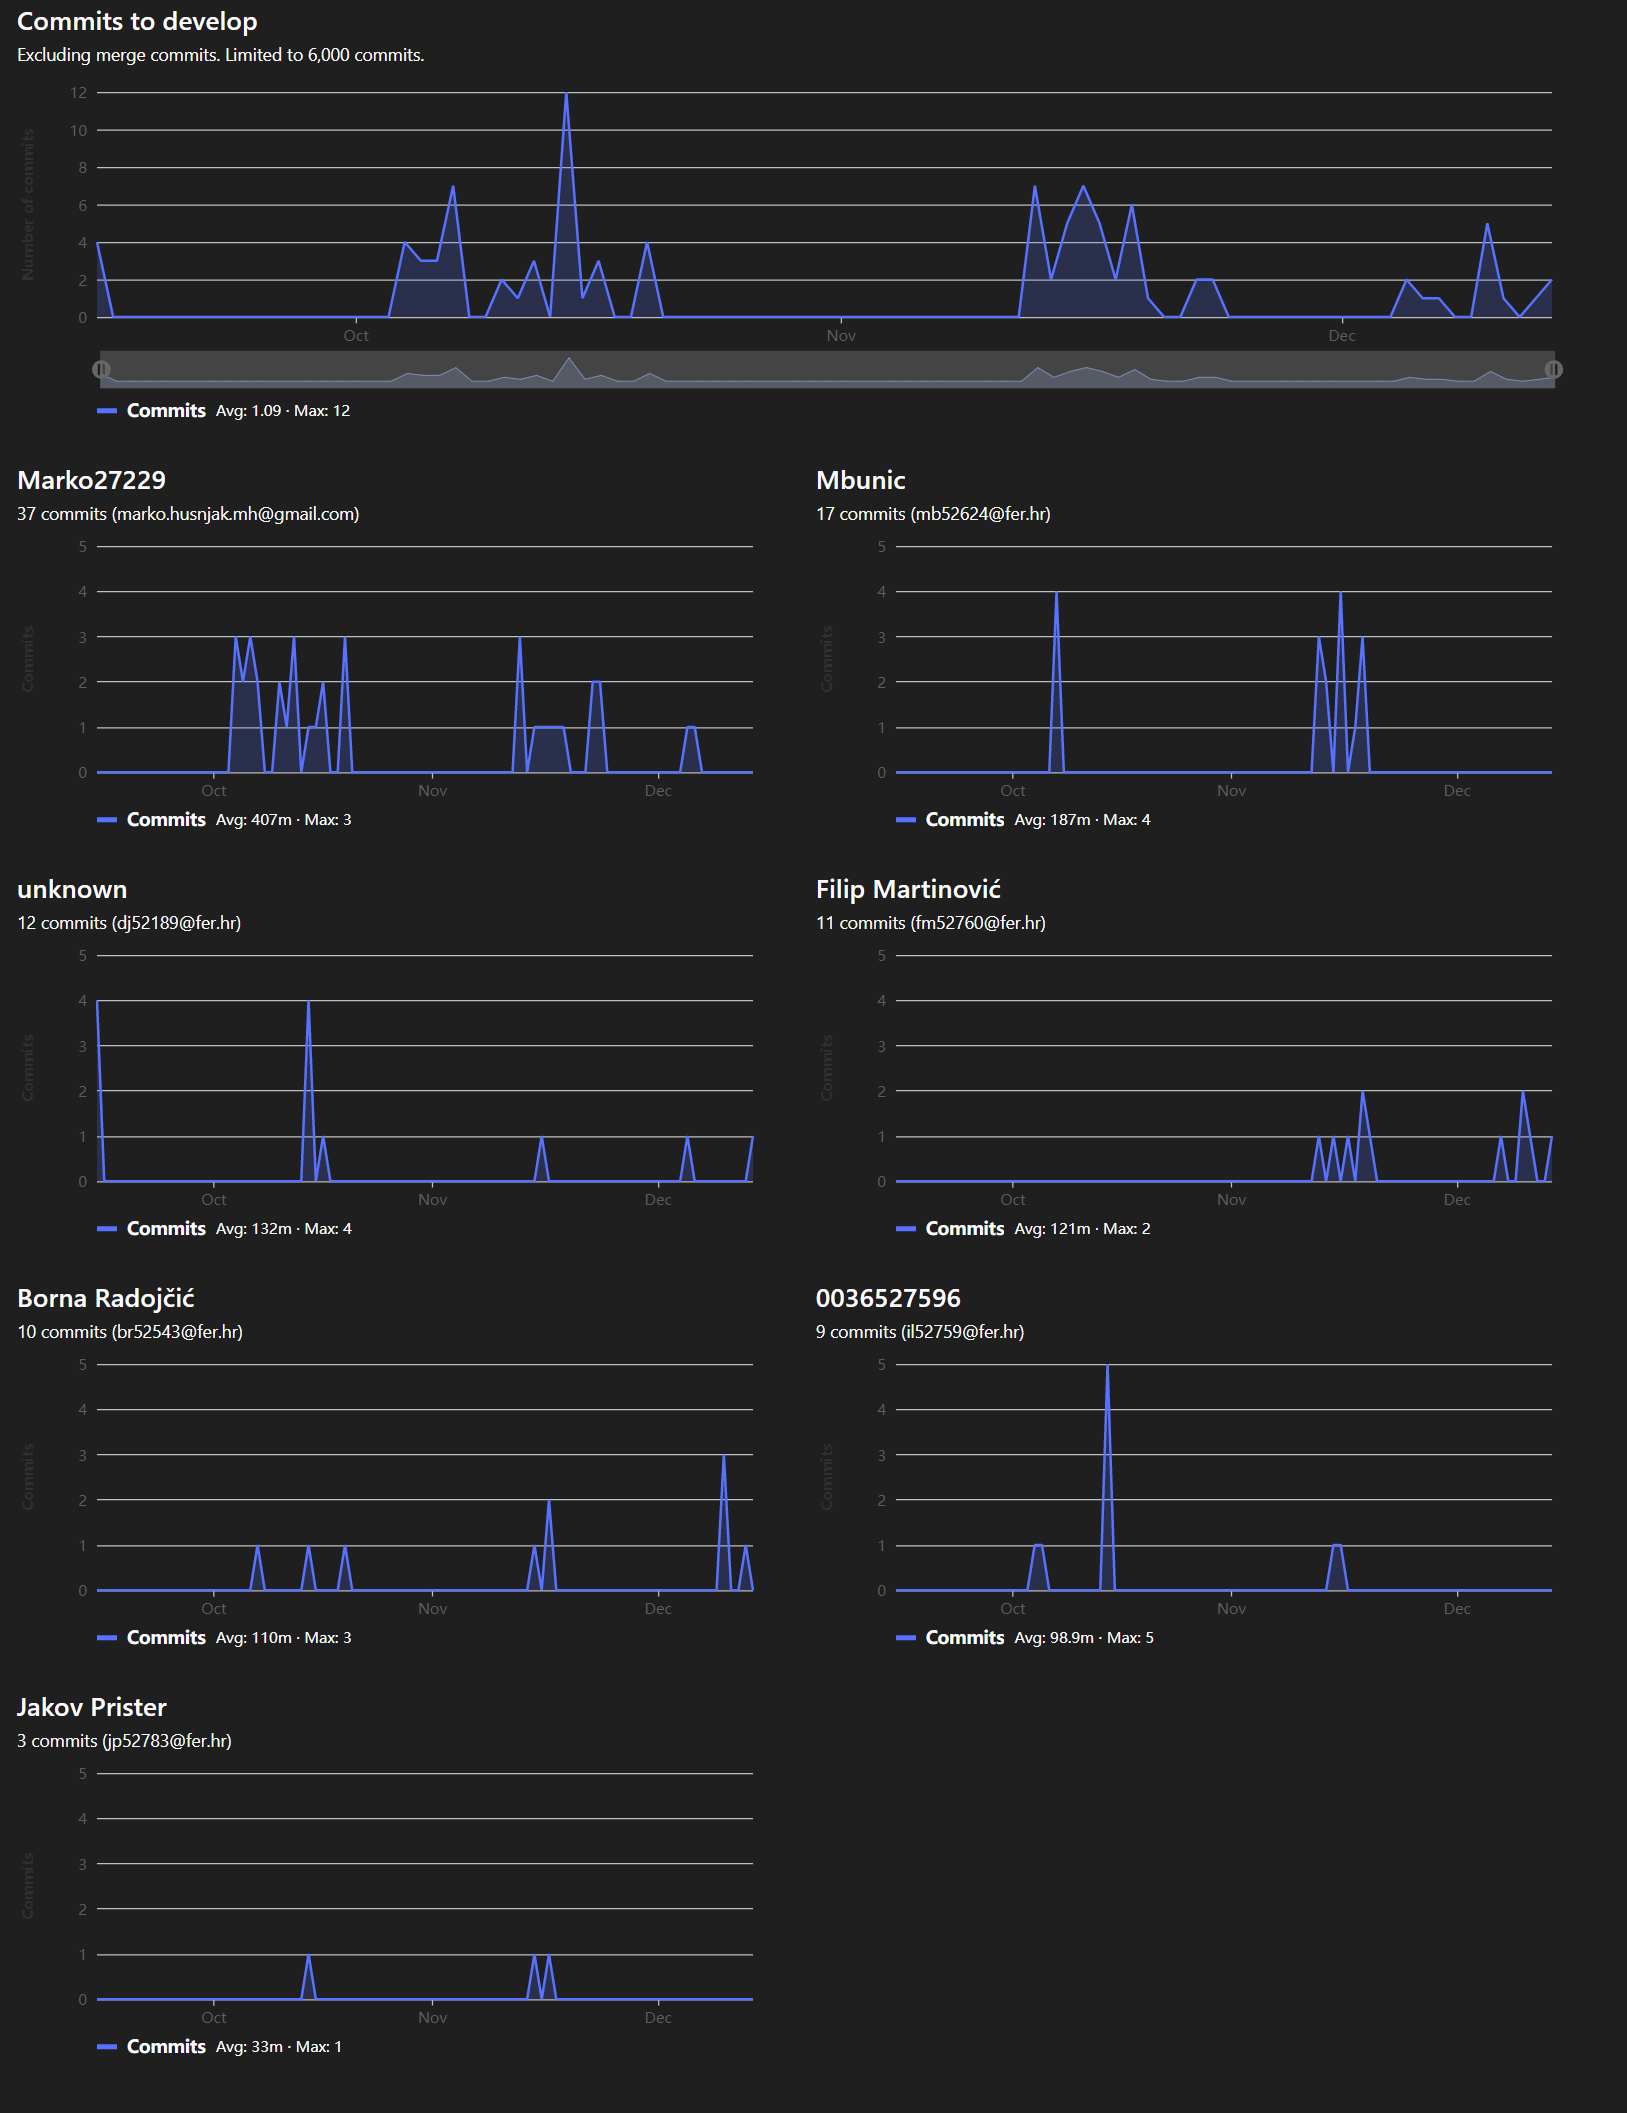
\includegraphics[scale=0.5]{./slike/develop.png}
			\caption{"Dijagram develop"}
			\label{fig:develop}
		\end{figure}
	
		\begin{figure}[H]
			\centering
			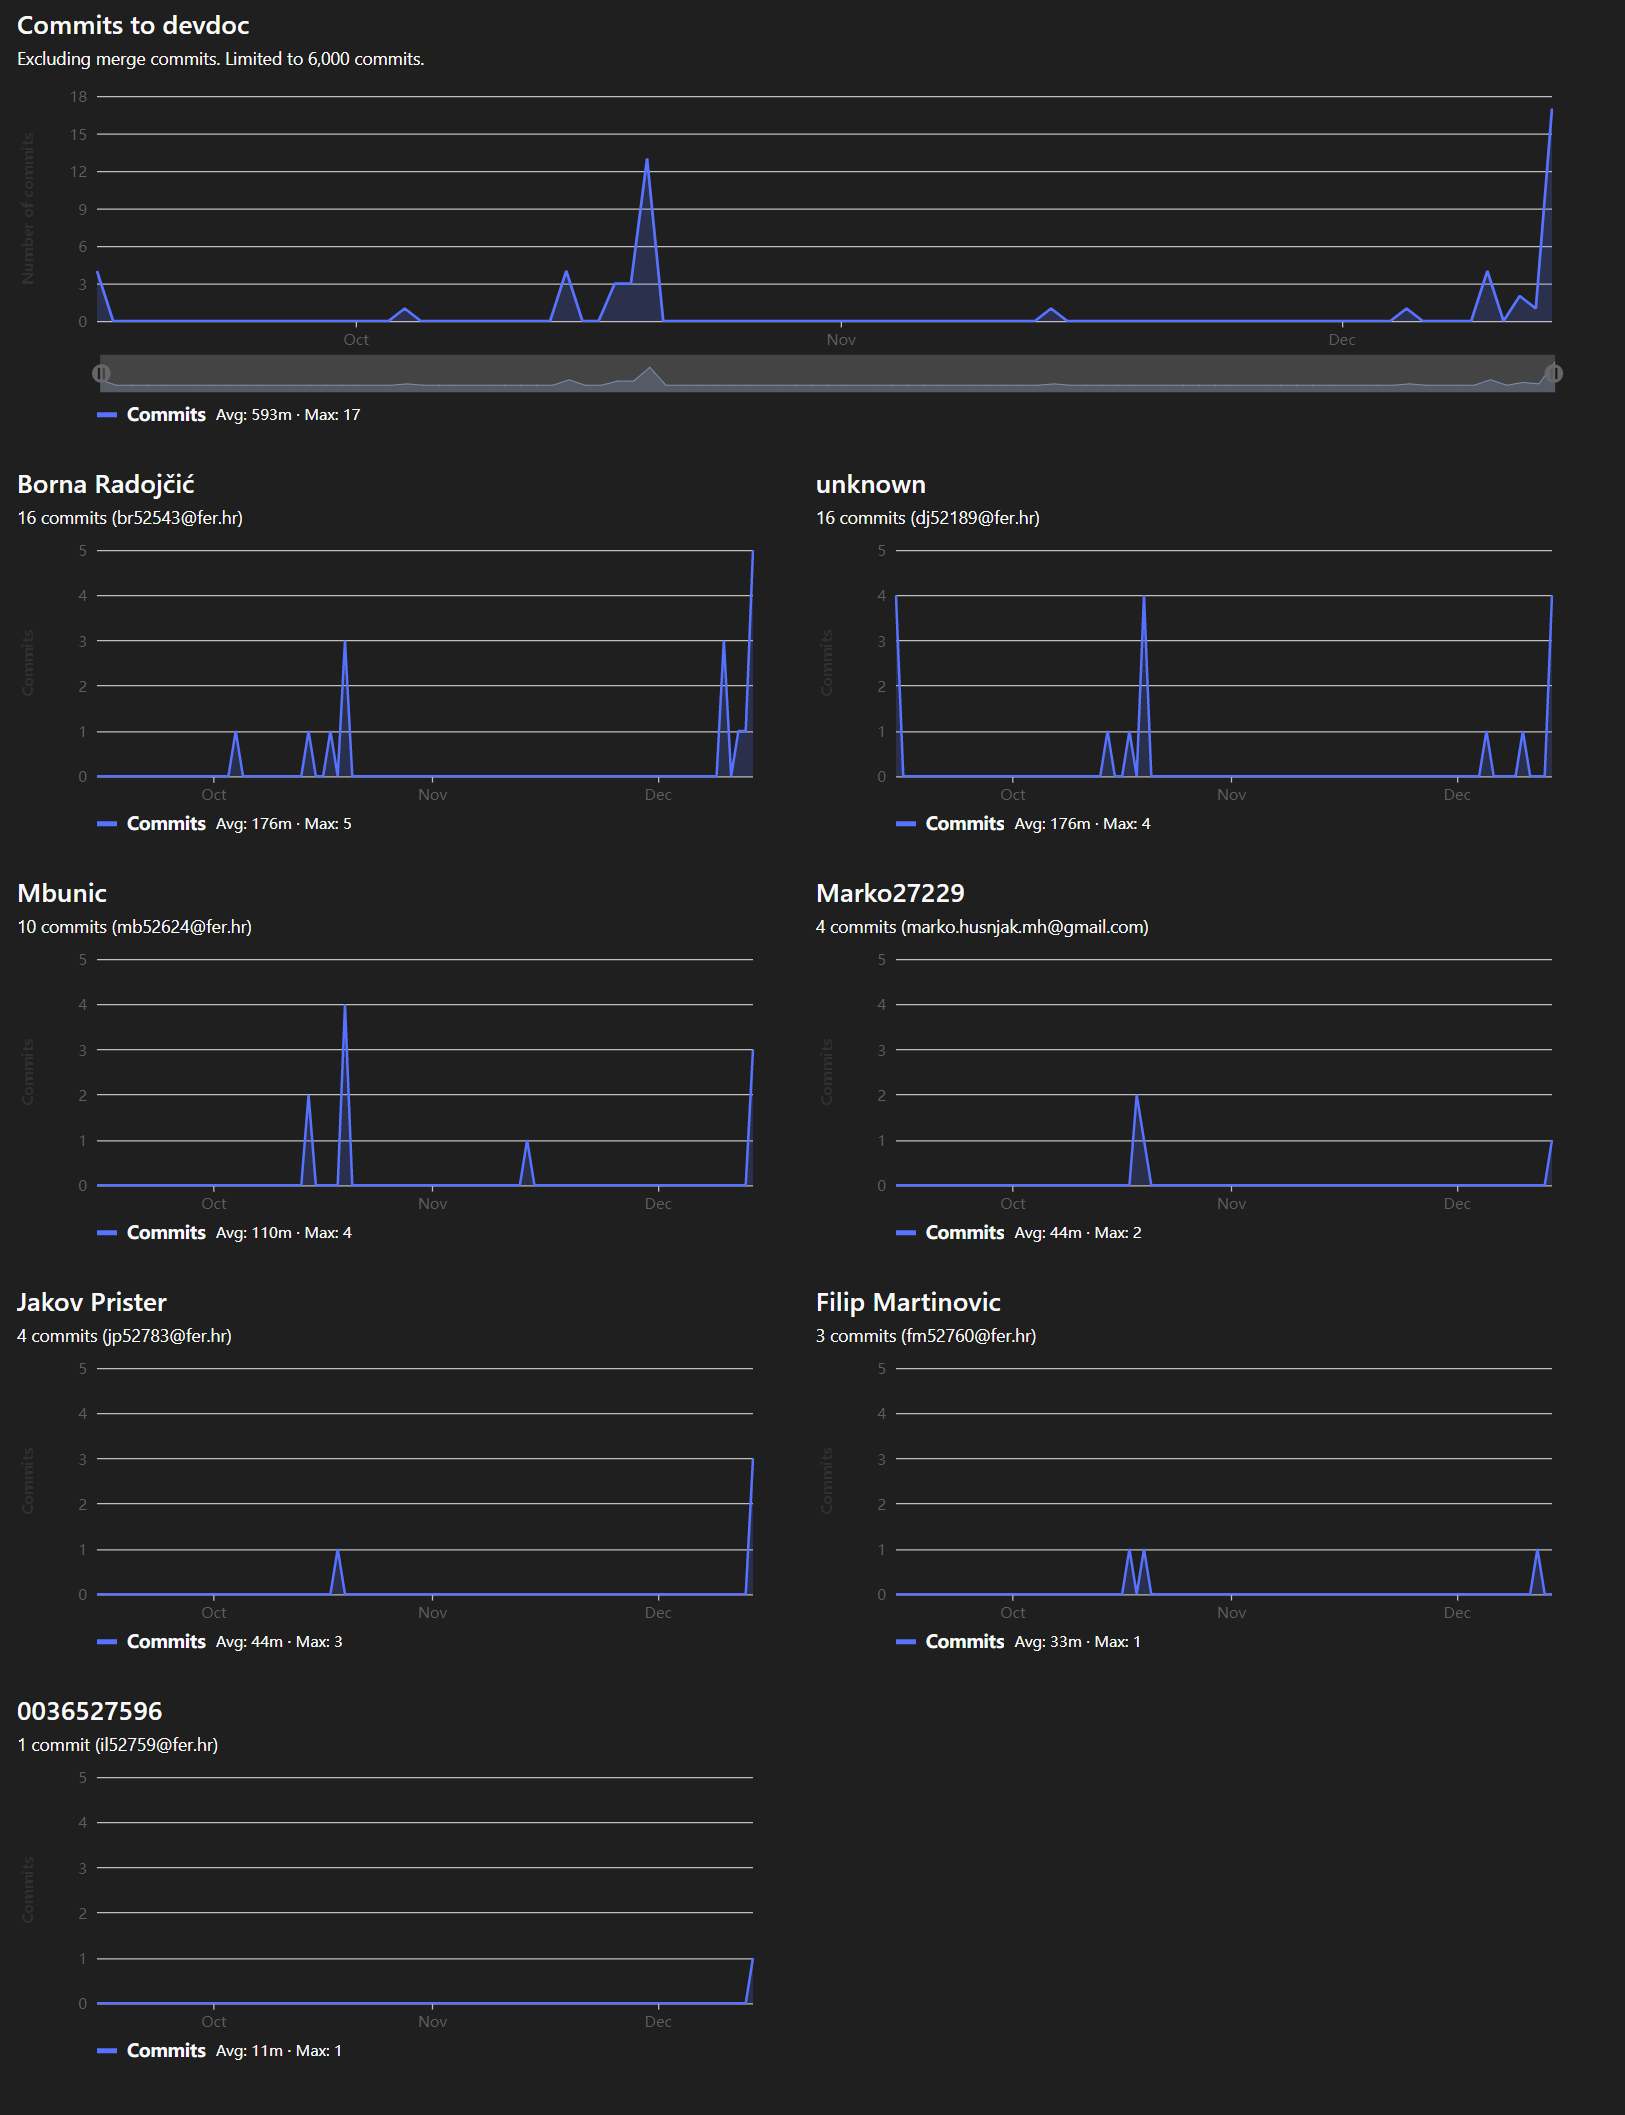
\includegraphics[scale=0.5]{./slike/devdoc.png}
			\caption{"Dijagram devdoc"}
			\label{fig:devdoc}
		\end{figure}
		
	